\documentclass[letterpaper,12pt]{article}
\usepackage[margin=.5in]{geometry}
\usepackage{tikz}
\usepackage{helvet}
\renewcommand{\familydefault}{\sfdefault}
\pagestyle{empty}
\pdfmapfile{+cm.map}
\pdfmapfile{+ps2pk35.map}
\setlength{\parindent}{0pt}
\hyphenpenalty=10000
\exhyphenpenalty=10000
\begin{document}
\null\begin{tikzpicture}[remember picture,overlay,x=1cm,y=1cm]
\begin{scope}[shift={(current page.north west)}]
\node[anchor=north west,inner sep=0pt,font=\fontsize{11.5}{13}\selectfont] at (1.4,-.72) {Week 33 / Prime-length necklaces / K--1};
\node[anchor=south west,inner sep=0pt,font=\fontsize{9}{11}\selectfont] at (1.4,-27.2) {Bellingham Math Circle / Week 33 / F33-K-v5};
\node[anchor=south east,inner sep=0pt,font=\fontsize{9}{11}\selectfont] at (20.15,-27.2) {1};
\begin{scope}[shift={(1.4,-1.65)}]
\node[anchor=north west,inner sep=0pt,align=left,text width=18.5cm,font=\fontsize{15}{18.9}\selectfont] at (0,0) {Read the beads going round from the start arrow. Rings are the same when turning makes them match.};
\draw[gray!65,line width=.7pt] (2.5,-4.6) circle (1.3cm);
\draw[fill=white] (2.5000,-3.3000) circle (0.29cm);
\node[font=\fontsize{12}{14}\selectfont,inner sep=1pt] at (2.5,-3.3) {A};
\draw[fill=white] (3.6258,-5.2500) circle (0.29cm);
\node[font=\fontsize{12}{14}\selectfont,inner sep=1pt] at (3.6258330249197703,-5.249999999999999) {A};
\draw[fill=gray!65] (1.3742,-5.2500) circle (0.29cm);
\node[font=\fontsize{12}{14}\selectfont,inner sep=1pt] at (1.37416697508023,-5.25) {B};
\draw[->,line width=.8pt] (2.5,-2.3499999999999996) -- (2.5,-2.8899999999999997);
\node[font=\fontsize{9}{11}\selectfont,inner sep=1pt] at (2.5,-2.1499999999999995) {start};
\draw[->,line width=.7pt] (0.9498,-3.7050) arc[start angle=150,end angle=110,radius=1.79cm];
\node[font=\fontsize{15}{17}\selectfont,inner sep=1pt] at (2.5,-6.65) {AAB};
\draw[gray!65,line width=.7pt] (8.5,-4.6) circle (1.3cm);
\draw[fill=white] (8.5000,-3.3000) circle (0.29cm);
\node[font=\fontsize{12}{14}\selectfont,inner sep=1pt] at (8.5,-3.3) {A};
\draw[fill=white] (9.6258,-5.2500) circle (0.29cm);
\node[font=\fontsize{12}{14}\selectfont,inner sep=1pt] at (9.625833024919771,-5.249999999999999) {A};
\draw[fill=gray!65] (7.3742,-5.2500) circle (0.29cm);
\node[font=\fontsize{12}{14}\selectfont,inner sep=1pt] at (7.37416697508023,-5.25) {B};
\draw[->,line width=.8pt] (10.448557158514987,-5.725) -- (9.98090344047139,-5.454999999999999);
\node[font=\fontsize{9}{11}\selectfont,inner sep=1pt] at (9.625833024919771,-5.8999999999999995) {start};
\draw[->,line width=.7pt] (6.9498,-3.7050) arc[start angle=150,end angle=110,radius=1.79cm];
\node[font=\fontsize{15}{17}\selectfont,inner sep=1pt] at (8.5,-6.65) {ABA};
\draw[gray!65,line width=.7pt] (14.5,-4.6) circle (1.3cm);
\draw[fill=white] (14.5000,-3.3000) circle (0.29cm);
\node[font=\fontsize{12}{14}\selectfont,inner sep=1pt] at (14.5,-3.3) {A};
\draw[fill=white] (15.6258,-5.2500) circle (0.29cm);
\node[font=\fontsize{12}{14}\selectfont,inner sep=1pt] at (15.625833024919771,-5.249999999999999) {A};
\draw[fill=gray!65] (13.3742,-5.2500) circle (0.29cm);
\node[font=\fontsize{12}{14}\selectfont,inner sep=1pt] at (13.37416697508023,-5.25) {B};
\draw[->,line width=.8pt] (12.551442841485013,-5.7250000000000005) -- (13.01909655952861,-5.455);
\node[font=\fontsize{9}{11}\selectfont,inner sep=1pt] at (13.37416697508023,-5.9) {start};
\draw[->,line width=.7pt] (12.9498,-3.7050) arc[start angle=150,end angle=110,radius=1.79cm];
\node[font=\fontsize{15}{17}\selectfont,inner sep=1pt] at (14.5,-6.65) {BAA};
\draw[->,line width=.8pt] (4.4,-4.6) -- (6.45,-4.6);
\draw[->,line width=.8pt] (10.4,-4.6) -- (12.45,-4.6);
\node[anchor=north west,inner sep=0pt,align=left,text width=3cm,font=\fontsize{10}{12.6}\selectfont] at (4.4,-3.1) {move start};
\node[anchor=north west,inner sep=0pt,align=left,text width=3cm,font=\fontsize{10}{12.6}\selectfont] at (10.4,-3.1) {move start};
\node[anchor=north west,inner sep=0pt,align=left,text width=18.6cm,font=\fontsize{15}{19.05}\selectfont] at (0,-7.8) {\textbf{Problem 1:} Make every different three-bead ring using A and B.};
\draw[gray!65,line width=.7pt] (2.7,-12.35) circle (1.75cm);
\draw[fill=white] (2.7000,-10.6000) circle (0.42cm);
\draw[fill=white] (4.2155,-13.2250) circle (0.42cm);
\draw[fill=white] (1.1845,-13.2250) circle (0.42cm);
\draw[->,line width=.7pt] (0.6475,-11.1650) arc[start angle=150,end angle=110,radius=2.37cm];
\draw[gray!45,line width=.35pt] (5.3,-11.2) -- (9.0,-11.2);
\draw[gray!45,line width=.35pt] (5.3,-12.35) -- (9.0,-12.35);
\draw[gray!45,line width=.35pt] (5.3,-13.5) -- (9.0,-13.5);
\draw[gray!65,line width=.7pt] (12.0,-12.35) circle (1.75cm);
\draw[fill=white] (12.0000,-10.6000) circle (0.42cm);
\draw[fill=white] (13.5155,-13.2250) circle (0.42cm);
\draw[fill=white] (10.4845,-13.2250) circle (0.42cm);
\draw[->,line width=.7pt] (9.9475,-11.1650) arc[start angle=150,end angle=110,radius=2.37cm];
\draw[gray!45,line width=.35pt] (14.6,-11.2) -- (18.5,-11.2);
\draw[gray!45,line width=.35pt] (14.6,-12.35) -- (18.5,-12.35);
\draw[gray!45,line width=.35pt] (14.6,-13.5) -- (18.5,-13.5);
\draw[gray!65,line width=.7pt] (2.7,-17.45) circle (1.75cm);
\draw[fill=white] (2.7000,-15.7000) circle (0.42cm);
\draw[fill=white] (4.2155,-18.3250) circle (0.42cm);
\draw[fill=white] (1.1845,-18.3250) circle (0.42cm);
\draw[->,line width=.7pt] (0.6475,-16.2650) arc[start angle=150,end angle=110,radius=2.37cm];
\draw[gray!45,line width=.35pt] (5.3,-16.3) -- (9.0,-16.3);
\draw[gray!45,line width=.35pt] (5.3,-17.45) -- (9.0,-17.45);
\draw[gray!45,line width=.35pt] (5.3,-18.6) -- (9.0,-18.6);
\draw[gray!65,line width=.7pt] (12.0,-17.45) circle (1.75cm);
\draw[fill=white] (12.0000,-15.7000) circle (0.42cm);
\draw[fill=white] (13.5155,-18.3250) circle (0.42cm);
\draw[fill=white] (10.4845,-18.3250) circle (0.42cm);
\draw[->,line width=.7pt] (9.9475,-16.2650) arc[start angle=150,end angle=110,radius=2.37cm];
\draw[gray!45,line width=.35pt] (14.6,-16.3) -- (18.5,-16.3);
\draw[gray!45,line width=.35pt] (14.6,-17.45) -- (18.5,-17.45);
\draw[gray!45,line width=.35pt] (14.6,-18.6) -- (18.5,-18.6);
\draw[gray!65,line width=.7pt] (2.7,-22.549999999999997) circle (1.75cm);
\draw[fill=white] (2.7000,-20.8000) circle (0.42cm);
\draw[fill=white] (4.2155,-23.4250) circle (0.42cm);
\draw[fill=white] (1.1845,-23.4250) circle (0.42cm);
\draw[->,line width=.7pt] (0.6475,-21.3650) arc[start angle=150,end angle=110,radius=2.37cm];
\draw[gray!45,line width=.35pt] (5.3,-21.4) -- (9.0,-21.4);
\draw[gray!45,line width=.35pt] (5.3,-22.549999999999997) -- (9.0,-22.549999999999997);
\draw[gray!45,line width=.35pt] (5.3,-23.7) -- (9.0,-23.7);
\draw[gray!65,line width=.7pt] (12.0,-22.549999999999997) circle (1.75cm);
\draw[fill=white] (12.0000,-20.8000) circle (0.42cm);
\draw[fill=white] (13.5155,-23.4250) circle (0.42cm);
\draw[fill=white] (10.4845,-23.4250) circle (0.42cm);
\draw[->,line width=.7pt] (9.9475,-21.3650) arc[start angle=150,end angle=110,radius=2.37cm];
\draw[gray!45,line width=.35pt] (14.6,-21.4) -- (18.5,-21.4);
\draw[gray!45,line width=.35pt] (14.6,-22.549999999999997) -- (18.5,-22.549999999999997);
\draw[gray!45,line width=.35pt] (14.6,-23.7) -- (18.5,-23.7);\end{scope}\end{scope}\end{tikzpicture}
\newpage
\null\begin{tikzpicture}[remember picture,overlay,x=1cm,y=1cm]
\begin{scope}[shift={(current page.north west)}]
\node[anchor=north west,inner sep=0pt,font=\fontsize{11.5}{13}\selectfont] at (1.4,-.72) {Week 33 / Prime-length necklaces / K--1};
\node[anchor=south west,inner sep=0pt,font=\fontsize{9}{11}\selectfont] at (1.4,-27.2) {Bellingham Math Circle / Week 33 / F33-K-v5};
\node[anchor=south east,inner sep=0pt,font=\fontsize{9}{11}\selectfont] at (20.15,-27.2) {2};
\begin{scope}[shift={(1.4,-1.65)}]
\node[anchor=north west,inner sep=0pt,align=left,text width=18.6cm,font=\fontsize{14}{17.78}\selectfont] at (0,0) {\textbf{Problem 2:} Put cards in the same group when they make the same ring. Do all groups have the same number of cards?};
\draw[line width=.65pt] (0.0,-2.2) rectangle (9.25,-7.4);
\draw[gray!65,line width=.7pt] (4.625,-5.15) circle (1.35cm);
\draw[fill=white] (4.6250,-3.8000) circle (0.36cm);
\node[font=\fontsize{12}{14}\selectfont,inner sep=1pt] at (4.625,-3.8000000000000003) {A};
\draw[fill=white] (5.7941,-5.8250) circle (0.36cm);
\node[font=\fontsize{12}{14}\selectfont,inner sep=1pt] at (5.794134295108992,-5.825) {A};
\draw[fill=white] (3.4559,-5.8250) circle (0.36cm);
\node[font=\fontsize{12}{14}\selectfont,inner sep=1pt] at (3.455865704891008,-5.825000000000001) {A};
\draw[->,line width=.8pt] (4.625,-2.8500000000000005) -- (4.625,-3.3200000000000003);
\node[font=\fontsize{9}{11}\selectfont,inner sep=1pt] at (4.625,-2.6500000000000004) {start};
\draw[->,line width=.7pt] (2.9709,-4.1950) arc[start angle=150,end angle=110,radius=1.91cm];
\node[font=\fontsize{9}{11}\selectfont,inner sep=1pt] at (8.95,-2.5) {1};
\draw[line width=.65pt] (9.25,-2.2) rectangle (18.5,-7.4);
\draw[gray!65,line width=.7pt] (13.875,-5.15) circle (1.35cm);
\draw[fill=white] (13.8750,-3.8000) circle (0.36cm);
\node[font=\fontsize{12}{14}\selectfont,inner sep=1pt] at (13.875,-3.8000000000000003) {A};
\draw[fill=white] (15.0441,-5.8250) circle (0.36cm);
\node[font=\fontsize{12}{14}\selectfont,inner sep=1pt] at (15.044134295108993,-5.825) {A};
\draw[fill=gray!65] (12.7059,-5.8250) circle (0.36cm);
\node[font=\fontsize{12}{14}\selectfont,inner sep=1pt] at (12.705865704891007,-5.825000000000001) {B};
\draw[->,line width=.8pt] (13.875,-2.8500000000000005) -- (13.875,-3.3200000000000003);
\node[font=\fontsize{9}{11}\selectfont,inner sep=1pt] at (13.875,-2.6500000000000004) {start};
\draw[->,line width=.7pt] (12.2209,-4.1950) arc[start angle=150,end angle=110,radius=1.91cm];
\node[font=\fontsize{9}{11}\selectfont,inner sep=1pt] at (18.2,-2.5) {2};
\draw[line width=.65pt] (0.0,-7.4) rectangle (9.25,-12.600000000000001);
\draw[gray!65,line width=.7pt] (4.625,-10.35) circle (1.35cm);
\draw[fill=white] (4.6250,-9.0000) circle (0.36cm);
\node[font=\fontsize{12}{14}\selectfont,inner sep=1pt] at (4.625,-9.0) {A};
\draw[fill=gray!65] (5.7941,-11.0250) circle (0.36cm);
\node[font=\fontsize{12}{14}\selectfont,inner sep=1pt] at (5.794134295108992,-11.024999999999999) {B};
\draw[fill=white] (3.4559,-11.0250) circle (0.36cm);
\node[font=\fontsize{12}{14}\selectfont,inner sep=1pt] at (3.455865704891008,-11.025) {A};
\draw[->,line width=.8pt] (4.625,-8.05) -- (4.625,-8.52);
\node[font=\fontsize{9}{11}\selectfont,inner sep=1pt] at (4.625,-7.8500000000000005) {start};
\draw[->,line width=.7pt] (2.9709,-9.3950) arc[start angle=150,end angle=110,radius=1.91cm];
\node[font=\fontsize{9}{11}\selectfont,inner sep=1pt] at (8.95,-7.7) {3};
\draw[line width=.65pt] (9.25,-7.4) rectangle (18.5,-12.600000000000001);
\draw[gray!65,line width=.7pt] (13.875,-10.35) circle (1.35cm);
\draw[fill=white] (13.8750,-9.0000) circle (0.36cm);
\node[font=\fontsize{12}{14}\selectfont,inner sep=1pt] at (13.875,-9.0) {A};
\draw[fill=gray!65] (15.0441,-11.0250) circle (0.36cm);
\node[font=\fontsize{12}{14}\selectfont,inner sep=1pt] at (15.044134295108993,-11.024999999999999) {B};
\draw[fill=gray!65] (12.7059,-11.0250) circle (0.36cm);
\node[font=\fontsize{12}{14}\selectfont,inner sep=1pt] at (12.705865704891007,-11.025) {B};
\draw[->,line width=.8pt] (13.875,-8.05) -- (13.875,-8.52);
\node[font=\fontsize{9}{11}\selectfont,inner sep=1pt] at (13.875,-7.8500000000000005) {start};
\draw[->,line width=.7pt] (12.2209,-9.3950) arc[start angle=150,end angle=110,radius=1.91cm];
\node[font=\fontsize{9}{11}\selectfont,inner sep=1pt] at (18.2,-7.7) {4};
\draw[line width=.65pt] (0.0,-12.600000000000001) rectangle (9.25,-17.8);
\draw[gray!65,line width=.7pt] (4.625,-15.55) circle (1.35cm);
\draw[fill=gray!65] (4.6250,-14.2000) circle (0.36cm);
\node[font=\fontsize{12}{14}\selectfont,inner sep=1pt] at (4.625,-14.200000000000001) {B};
\draw[fill=white] (5.7941,-16.2250) circle (0.36cm);
\node[font=\fontsize{12}{14}\selectfont,inner sep=1pt] at (5.794134295108992,-16.225) {A};
\draw[fill=white] (3.4559,-16.2250) circle (0.36cm);
\node[font=\fontsize{12}{14}\selectfont,inner sep=1pt] at (3.455865704891008,-16.225) {A};
\draw[->,line width=.8pt] (4.625,-13.25) -- (4.625,-13.72);
\node[font=\fontsize{9}{11}\selectfont,inner sep=1pt] at (4.625,-13.05) {start};
\draw[->,line width=.7pt] (2.9709,-14.5950) arc[start angle=150,end angle=110,radius=1.91cm];
\node[font=\fontsize{9}{11}\selectfont,inner sep=1pt] at (8.95,-12.900000000000002) {5};
\draw[line width=.65pt] (9.25,-12.600000000000001) rectangle (18.5,-17.8);
\draw[gray!65,line width=.7pt] (13.875,-15.55) circle (1.35cm);
\draw[fill=gray!65] (13.8750,-14.2000) circle (0.36cm);
\node[font=\fontsize{12}{14}\selectfont,inner sep=1pt] at (13.875,-14.200000000000001) {B};
\draw[fill=white] (15.0441,-16.2250) circle (0.36cm);
\node[font=\fontsize{12}{14}\selectfont,inner sep=1pt] at (15.044134295108993,-16.225) {A};
\draw[fill=gray!65] (12.7059,-16.2250) circle (0.36cm);
\node[font=\fontsize{12}{14}\selectfont,inner sep=1pt] at (12.705865704891007,-16.225) {B};
\draw[->,line width=.8pt] (13.875,-13.25) -- (13.875,-13.72);
\node[font=\fontsize{9}{11}\selectfont,inner sep=1pt] at (13.875,-13.05) {start};
\draw[->,line width=.7pt] (12.2209,-14.5950) arc[start angle=150,end angle=110,radius=1.91cm];
\node[font=\fontsize{9}{11}\selectfont,inner sep=1pt] at (18.2,-12.900000000000002) {6};
\draw[line width=.65pt] (0.0,-17.8) rectangle (9.25,-23.0);
\draw[gray!65,line width=.7pt] (4.625,-20.750000000000004) circle (1.35cm);
\draw[fill=gray!65] (4.6250,-19.4000) circle (0.36cm);
\node[font=\fontsize{12}{14}\selectfont,inner sep=1pt] at (4.625,-19.400000000000002) {B};
\draw[fill=gray!65] (5.7941,-21.4250) circle (0.36cm);
\node[font=\fontsize{12}{14}\selectfont,inner sep=1pt] at (5.794134295108992,-21.425000000000004) {B};
\draw[fill=white] (3.4559,-21.4250) circle (0.36cm);
\node[font=\fontsize{12}{14}\selectfont,inner sep=1pt] at (3.455865704891008,-21.425000000000004) {A};
\draw[->,line width=.8pt] (4.625,-18.450000000000003) -- (4.625,-18.92);
\node[font=\fontsize{9}{11}\selectfont,inner sep=1pt] at (4.625,-18.250000000000004) {start};
\draw[->,line width=.7pt] (2.9709,-19.7950) arc[start angle=150,end angle=110,radius=1.91cm];
\node[font=\fontsize{9}{11}\selectfont,inner sep=1pt] at (8.95,-18.1) {7};
\draw[line width=.65pt] (9.25,-17.8) rectangle (18.5,-23.0);
\draw[gray!65,line width=.7pt] (13.875,-20.750000000000004) circle (1.35cm);
\draw[fill=gray!65] (13.8750,-19.4000) circle (0.36cm);
\node[font=\fontsize{12}{14}\selectfont,inner sep=1pt] at (13.875,-19.400000000000002) {B};
\draw[fill=gray!65] (15.0441,-21.4250) circle (0.36cm);
\node[font=\fontsize{12}{14}\selectfont,inner sep=1pt] at (15.044134295108993,-21.425000000000004) {B};
\draw[fill=gray!65] (12.7059,-21.4250) circle (0.36cm);
\node[font=\fontsize{12}{14}\selectfont,inner sep=1pt] at (12.705865704891007,-21.425000000000004) {B};
\draw[->,line width=.8pt] (13.875,-18.450000000000003) -- (13.875,-18.92);
\node[font=\fontsize{9}{11}\selectfont,inner sep=1pt] at (13.875,-18.250000000000004) {start};
\draw[->,line width=.7pt] (12.2209,-19.7950) arc[start angle=150,end angle=110,radius=1.91cm];
\node[font=\fontsize{9}{11}\selectfont,inner sep=1pt] at (18.2,-18.1) {8};\end{scope}\end{scope}\end{tikzpicture}
\newpage
\null\begin{tikzpicture}[remember picture,overlay,x=1cm,y=1cm]
\begin{scope}[shift={(current page.north west)}]
\node[anchor=north west,inner sep=0pt,font=\fontsize{11.5}{13}\selectfont] at (1.4,-.72) {Week 33 / Prime-length necklaces / K--1};
\node[anchor=south west,inner sep=0pt,font=\fontsize{9}{11}\selectfont] at (1.4,-27.2) {Bellingham Math Circle / Week 33 / F33-K-v5};
\node[anchor=south east,inner sep=0pt,font=\fontsize{9}{11}\selectfont] at (20.15,-27.2) {3};
\begin{scope}[shift={(1.4,-1.65)}]
\node[anchor=north west,inner sep=0pt,align=left,text width=18.6cm,font=\fontsize{15}{19.05}\selectfont] at (0,0) {\textbf{Problem 3:} Find every different four-bead ring with two A beads and two B beads.};
\draw[gray!65,line width=.7pt] (4.4,-8) circle (3.65cm);
\draw[fill=white] (4.4000,-4.3500) circle (0.42cm);
\draw[fill=white] (8.0500,-8.0000) circle (0.42cm);
\draw[fill=white] (4.4000,-11.6500) circle (0.42cm);
\draw[fill=white] (0.7500,-8.0000) circle (0.42cm);
\draw[->,line width=.7pt] (0.7021,-5.8650) arc[start angle=150,end angle=110,radius=4.2700000000000005cm];
\draw[gray!65,line width=.7pt] (14.0,-8) circle (3.65cm);
\draw[fill=white] (14.0000,-4.3500) circle (0.42cm);
\draw[fill=white] (17.6500,-8.0000) circle (0.42cm);
\draw[fill=white] (14.0000,-11.6500) circle (0.42cm);
\draw[fill=white] (10.3500,-8.0000) circle (0.42cm);
\draw[->,line width=.7pt] (10.3021,-5.8650) arc[start angle=150,end angle=110,radius=4.2700000000000005cm];
\draw[gray!65,line width=.7pt] (4.4,-18) circle (3.65cm);
\draw[fill=white] (4.4000,-14.3500) circle (0.42cm);
\draw[fill=white] (8.0500,-18.0000) circle (0.42cm);
\draw[fill=white] (4.4000,-21.6500) circle (0.42cm);
\draw[fill=white] (0.7500,-18.0000) circle (0.42cm);
\draw[->,line width=.7pt] (0.7021,-15.8650) arc[start angle=150,end angle=110,radius=4.2700000000000005cm];
\draw[gray!65,line width=.7pt] (14.0,-18) circle (3.65cm);
\draw[fill=white] (14.0000,-14.3500) circle (0.42cm);
\draw[fill=white] (17.6500,-18.0000) circle (0.42cm);
\draw[fill=white] (14.0000,-21.6500) circle (0.42cm);
\draw[fill=white] (10.3500,-18.0000) circle (0.42cm);
\draw[->,line width=.7pt] (10.3021,-15.8650) arc[start angle=150,end angle=110,radius=4.2700000000000005cm];\end{scope}\end{scope}\end{tikzpicture}
\newpage
\null\begin{tikzpicture}[remember picture,overlay,x=1cm,y=1cm]
\begin{scope}[shift={(current page.north west)}]
\node[anchor=north west,inner sep=0pt,font=\fontsize{11.5}{13}\selectfont] at (1.4,-.72) {Week 33 / Prime-length necklaces / K--1};
\node[anchor=south west,inner sep=0pt,font=\fontsize{9}{11}\selectfont] at (1.4,-27.2) {Bellingham Math Circle / Week 33 / F33-K-v5};
\node[anchor=south east,inner sep=0pt,font=\fontsize{9}{11}\selectfont] at (20.15,-27.2) {4};
\begin{scope}[shift={(1.4,-1.65)}]
\node[anchor=north west,inner sep=0pt,align=left,text width=18.6cm,font=\fontsize{15}{19.05}\selectfont] at (0,0) {\textbf{Problem 4:} Make four-bead rings with one, two, three or four different readouts. Which are possible?};
\draw[gray!65,line width=.7pt] (4.4,-8) circle (3.65cm);
\draw[fill=white] (4.4000,-4.3500) circle (0.42cm);
\draw[fill=white] (8.0500,-8.0000) circle (0.42cm);
\draw[fill=white] (4.4000,-11.6500) circle (0.42cm);
\draw[fill=white] (0.7500,-8.0000) circle (0.42cm);
\draw[->,line width=.7pt] (0.7021,-5.8650) arc[start angle=150,end angle=110,radius=4.2700000000000005cm];
\draw[gray!65,line width=.7pt] (14.0,-8) circle (3.65cm);
\draw[fill=white] (14.0000,-4.3500) circle (0.42cm);
\draw[fill=white] (17.6500,-8.0000) circle (0.42cm);
\draw[fill=white] (14.0000,-11.6500) circle (0.42cm);
\draw[fill=white] (10.3500,-8.0000) circle (0.42cm);
\draw[->,line width=.7pt] (10.3021,-5.8650) arc[start angle=150,end angle=110,radius=4.2700000000000005cm];
\draw[gray!65,line width=.7pt] (4.4,-18) circle (3.65cm);
\draw[fill=white] (4.4000,-14.3500) circle (0.42cm);
\draw[fill=white] (8.0500,-18.0000) circle (0.42cm);
\draw[fill=white] (4.4000,-21.6500) circle (0.42cm);
\draw[fill=white] (0.7500,-18.0000) circle (0.42cm);
\draw[->,line width=.7pt] (0.7021,-15.8650) arc[start angle=150,end angle=110,radius=4.2700000000000005cm];
\draw[gray!65,line width=.7pt] (14.0,-18) circle (3.65cm);
\draw[fill=white] (14.0000,-14.3500) circle (0.42cm);
\draw[fill=white] (17.6500,-18.0000) circle (0.42cm);
\draw[fill=white] (14.0000,-21.6500) circle (0.42cm);
\draw[fill=white] (10.3500,-18.0000) circle (0.42cm);
\draw[->,line width=.7pt] (10.3021,-15.8650) arc[start angle=150,end angle=110,radius=4.2700000000000005cm];\end{scope}\end{scope}\end{tikzpicture}
\newpage
\null\begin{tikzpicture}[remember picture,overlay,x=1cm,y=1cm]
\begin{scope}[shift={(current page.north west)}]
\node[anchor=north west,inner sep=0pt,font=\fontsize{11.5}{13}\selectfont] at (1.4,-.72) {Week 33 / Prime-length necklaces / K--1};
\node[anchor=south west,inner sep=0pt,font=\fontsize{9}{11}\selectfont] at (1.4,-27.2) {Bellingham Math Circle / Week 33 / F33-K-v5};
\node[anchor=south east,inner sep=0pt,font=\fontsize{9}{11}\selectfont] at (20.15,-27.2) {5};
\begin{scope}[shift={(1.4,-1.65)}]
\node[anchor=north west,inner sep=0pt,align=left,text width=18.6cm,font=\fontsize{15}{19.05}\selectfont] at (0,0) {\textbf{Problem 5:} Find every different five-bead ring with two A beads and three B beads.};
\draw[gray!65,line width=.7pt] (4.4,-8) circle (3.65cm);
\draw[fill=white] (4.4000,-4.3500) circle (0.42cm);
\draw[fill=white] (7.8714,-6.8721) circle (0.42cm);
\draw[fill=white] (6.5454,-10.9529) circle (0.42cm);
\draw[fill=white] (2.2546,-10.9529) circle (0.42cm);
\draw[fill=white] (0.9286,-6.8721) circle (0.42cm);
\draw[->,line width=.7pt] (0.7021,-5.8650) arc[start angle=150,end angle=110,radius=4.2700000000000005cm];
\draw[gray!65,line width=.7pt] (14.0,-8) circle (3.65cm);
\draw[fill=white] (14.0000,-4.3500) circle (0.42cm);
\draw[fill=white] (17.4714,-6.8721) circle (0.42cm);
\draw[fill=white] (16.1454,-10.9529) circle (0.42cm);
\draw[fill=white] (11.8546,-10.9529) circle (0.42cm);
\draw[fill=white] (10.5286,-6.8721) circle (0.42cm);
\draw[->,line width=.7pt] (10.3021,-5.8650) arc[start angle=150,end angle=110,radius=4.2700000000000005cm];
\draw[gray!65,line width=.7pt] (4.4,-18) circle (3.65cm);
\draw[fill=white] (4.4000,-14.3500) circle (0.42cm);
\draw[fill=white] (7.8714,-16.8721) circle (0.42cm);
\draw[fill=white] (6.5454,-20.9529) circle (0.42cm);
\draw[fill=white] (2.2546,-20.9529) circle (0.42cm);
\draw[fill=white] (0.9286,-16.8721) circle (0.42cm);
\draw[->,line width=.7pt] (0.7021,-15.8650) arc[start angle=150,end angle=110,radius=4.2700000000000005cm];
\draw[gray!65,line width=.7pt] (14.0,-18) circle (3.65cm);
\draw[fill=white] (14.0000,-14.3500) circle (0.42cm);
\draw[fill=white] (17.4714,-16.8721) circle (0.42cm);
\draw[fill=white] (16.1454,-20.9529) circle (0.42cm);
\draw[fill=white] (11.8546,-20.9529) circle (0.42cm);
\draw[fill=white] (10.5286,-16.8721) circle (0.42cm);
\draw[->,line width=.7pt] (10.3021,-15.8650) arc[start angle=150,end angle=110,radius=4.2700000000000005cm];\end{scope}\end{scope}\end{tikzpicture}
\newpage
\null\begin{tikzpicture}[remember picture,overlay,x=1cm,y=1cm]
\begin{scope}[shift={(current page.north west)}]
\node[anchor=north west,inner sep=0pt,font=\fontsize{11.5}{13}\selectfont] at (1.4,-.72) {Week 33 / Prime-length necklaces / K--1};
\node[anchor=south west,inner sep=0pt,font=\fontsize{9}{11}\selectfont] at (1.4,-27.2) {Bellingham Math Circle / Week 33 / F33-K-v5};
\node[anchor=south east,inner sep=0pt,font=\fontsize{9}{11}\selectfont] at (20.15,-27.2) {6};
\begin{scope}[shift={(1.4,-1.65)}]
\node[anchor=north west,inner sep=0pt,align=left,text width=18.6cm,font=\fontsize{15}{19.05}\selectfont] at (0,0) {\textbf{Problem 6:} Use both A and B on a six-bead ring. Find rings with two, three and six different readouts.};
\draw[gray!65,line width=.7pt] (4.4,-8) circle (3.65cm);
\draw[fill=white] (4.4000,-4.3500) circle (0.42cm);
\draw[fill=white] (7.5610,-6.1750) circle (0.42cm);
\draw[fill=white] (7.5610,-9.8250) circle (0.42cm);
\draw[fill=white] (4.4000,-11.6500) circle (0.42cm);
\draw[fill=white] (1.2390,-9.8250) circle (0.42cm);
\draw[fill=white] (1.2390,-6.1750) circle (0.42cm);
\draw[->,line width=.7pt] (0.7021,-5.8650) arc[start angle=150,end angle=110,radius=4.2700000000000005cm];
\draw[gray!65,line width=.7pt] (14.0,-8) circle (3.65cm);
\draw[fill=white] (14.0000,-4.3500) circle (0.42cm);
\draw[fill=white] (17.1610,-6.1750) circle (0.42cm);
\draw[fill=white] (17.1610,-9.8250) circle (0.42cm);
\draw[fill=white] (14.0000,-11.6500) circle (0.42cm);
\draw[fill=white] (10.8390,-9.8250) circle (0.42cm);
\draw[fill=white] (10.8390,-6.1750) circle (0.42cm);
\draw[->,line width=.7pt] (10.3021,-5.8650) arc[start angle=150,end angle=110,radius=4.2700000000000005cm];
\draw[gray!65,line width=.7pt] (4.4,-18) circle (3.65cm);
\draw[fill=white] (4.4000,-14.3500) circle (0.42cm);
\draw[fill=white] (7.5610,-16.1750) circle (0.42cm);
\draw[fill=white] (7.5610,-19.8250) circle (0.42cm);
\draw[fill=white] (4.4000,-21.6500) circle (0.42cm);
\draw[fill=white] (1.2390,-19.8250) circle (0.42cm);
\draw[fill=white] (1.2390,-16.1750) circle (0.42cm);
\draw[->,line width=.7pt] (0.7021,-15.8650) arc[start angle=150,end angle=110,radius=4.2700000000000005cm];
\draw[gray!65,line width=.7pt] (14.0,-18) circle (3.65cm);
\draw[fill=white] (14.0000,-14.3500) circle (0.42cm);
\draw[fill=white] (17.1610,-16.1750) circle (0.42cm);
\draw[fill=white] (17.1610,-19.8250) circle (0.42cm);
\draw[fill=white] (14.0000,-21.6500) circle (0.42cm);
\draw[fill=white] (10.8390,-19.8250) circle (0.42cm);
\draw[fill=white] (10.8390,-16.1750) circle (0.42cm);
\draw[->,line width=.7pt] (10.3021,-15.8650) arc[start angle=150,end angle=110,radius=4.2700000000000005cm];\end{scope}\end{scope}\end{tikzpicture}
\end{document}
